Un tremplin uniforme de \qty{\v{M}}{kg} et de \qty{\v{L}}{m} est retenu par deux supports : un boulon à l'extrémité gauche, qui peut tirer vers le bas, et un appui situé à \qty{\v{d}}{m} du boulon. Un plongeur de \qty{\v{m}}{kg} se tient immobile à l'extrémité droite.

\begin{center}
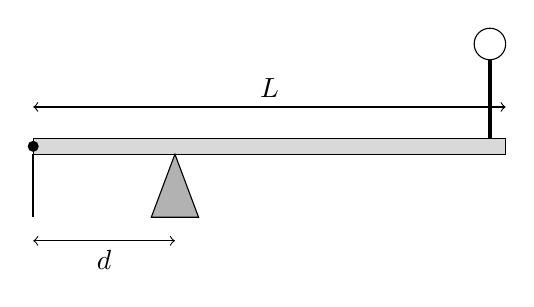
\begin{tikzpicture}[scale=1]
  \fill[gray!30] (0,0) rectangle (6,0.2); \draw (0,0) rectangle (6,0.2);
  \fill (0,0.1) circle (2pt); \draw[thick] (0,0) -- (0,-0.8);
  \draw[fill=gray!60] (1.8,0) -- (1.5,-0.8) -- (2.1,-0.8) -- cycle;
  \draw[very thick] (5.8,0.2) -- (5.8,1.2); \draw (5.8,1.4) circle (0.2);
  \draw[<->] (0,-1.1) -- node[below] {$d$} (1.8,-1.1);
  \draw[<->] (0,0.6) -- node[above] {$L$} (6,0.6);
\end{tikzpicture}
\end{center}

\begin{enumerate}[label=\alph*)]
    \item Déterminez la force exercée par l'appui sur le tremplin.
    \item Déterminez la force exercée par le boulon sur le tremplin.
\end{enumerate}
